\section{Security Analysis}
\label{sec:security}

The rest of this section describes the security properties of
enclaves, discussing the trade-offs made while trying to balance security with
backwards compatibility.

% Interactions with Paging: SDM S 42.4
% The Intel SGX access control itself is implemented as an extension to the
% three paging modes of Intel Architecture.

% Page-Based Access Control: SDM S 38.5

% ECREATE forces R, W, X to 0 in the page's EPCM. EADD also forces R/W/X to 0
% if the page type in SECINFO is PT_TCS (the only special type it can create).
%
%
% EPA doesn't read any SECINFO, and uses 0 for R, W, X.

% ERESUME can be replaced by normal EENTER, XRESTOR and accounting. Describe
% and argue against ERESUME.


% The use of the page version (nonce) as counter in AES-GCM makes it impossible
% for malicious system software to determine whether an EPC page's contents has
% changed between two evictions.
% However, the dirty bit in the EPC page's PTE will leak that information.

% According to the ECREATE pseudo-code in the Intel manual, EIDs are assigned
% using a counter that is atomically incremented on every ECREATE. This makes
% the field predictible to system software.


% The SGX instruction that evicts an EPC page, EWB, ensures that the VA slot it
% is supposed to write is unused.
% The VA unused slot check in EWB is unnecessary. Bad system software can only
% overwrite a version and impair its ability to restore a page.

Enclaves were designed to contain and protect the privacy-sensitive parts of an
application. All the code that handles private data must receive integrity
protection. Otherwise, a hostile environment could modify the code to leak
information about private data. Therefore, the SGX programming model prescribes
that code which accesses private data must be entirely contained inside an
enclave. Jumping into and out of enclave code must be performed explicitly
using the dedicated instructions \texttt{EENTER} and \texttt{EEXIT}.



\begin{figure}[hbt]
  \centering
  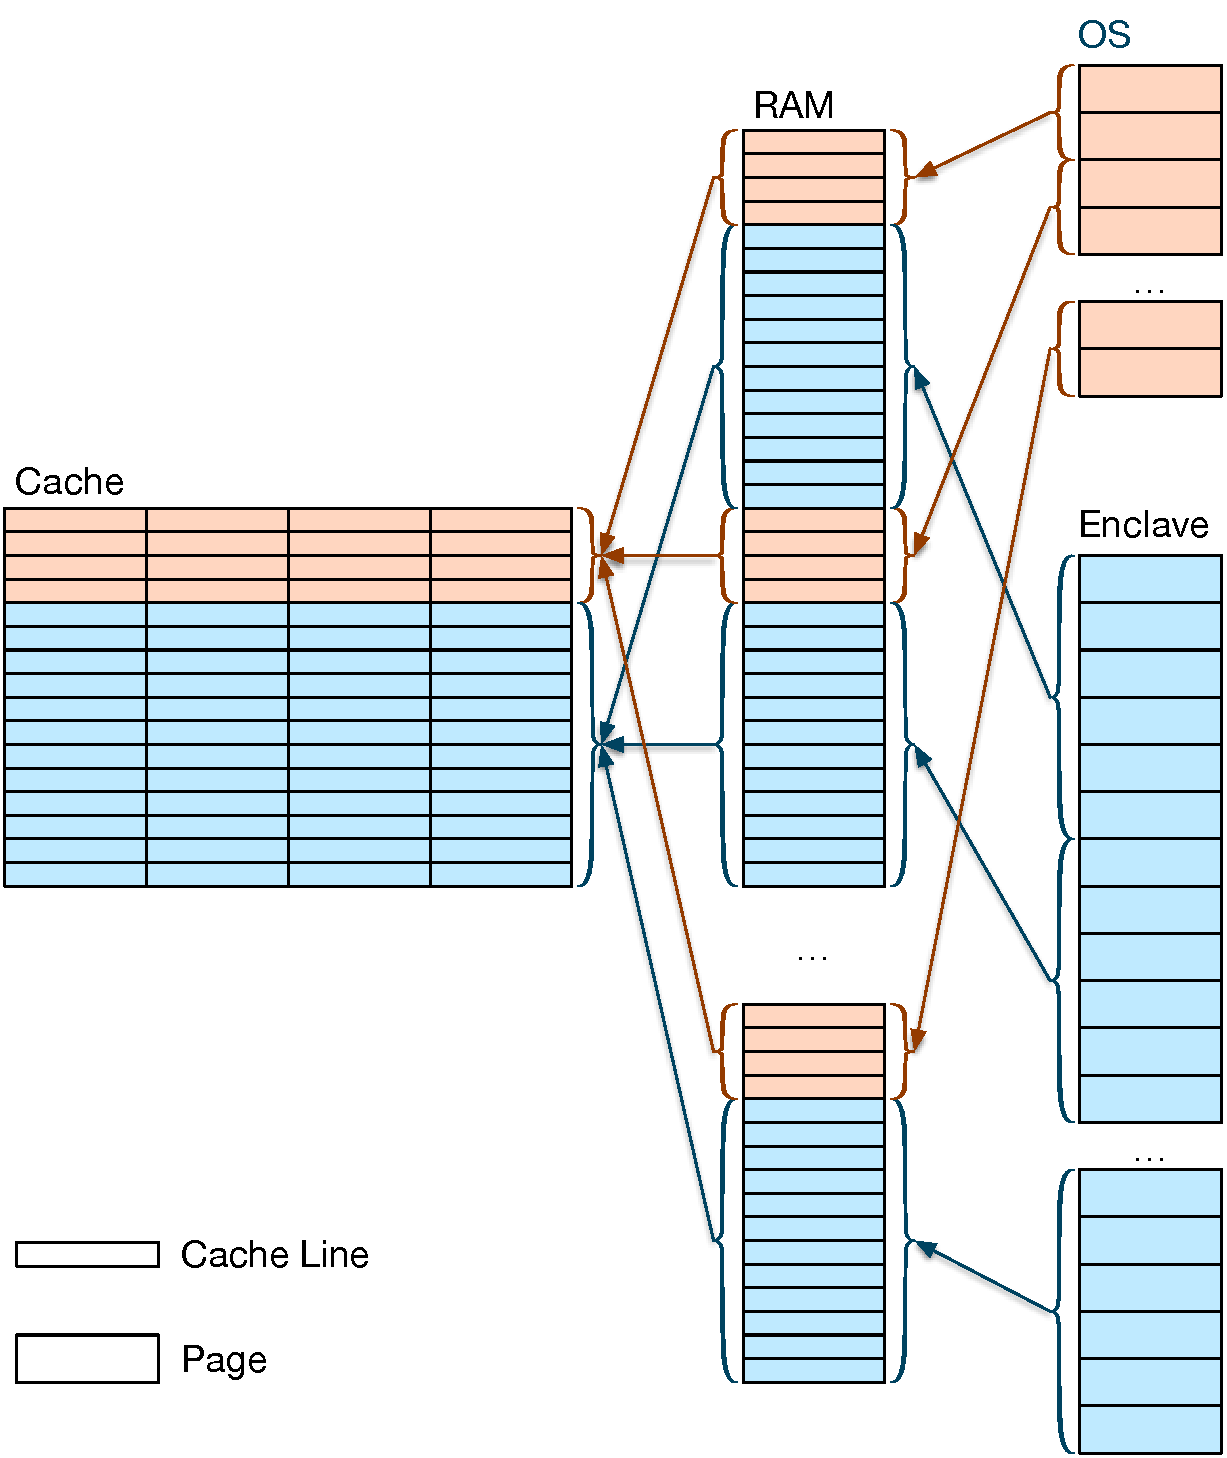
\includegraphics[width=85mm]{figures/cache_partitions.pdf}
  \caption{
    Cache partitioning between two applications. Each application has some
    cache sets allocated to it, and only uses RAM regions that map to its cache
    sets. When partitioning the L1 cache, applications have to follow this
    constraint themselves. When the L2 cache is partitioned, the OS can map the
    pages in an application's virtual address space to the RAM regions that the
    application can use, so applications are oblivious to the cache
    partitioning.
  }
  \label{fig:cache_partitions}
\end{figure}


\subsection{DOS Prevention}
% NOTE: This is a slightly edited answer to a question we received.

SGX enclaves execute at the lowest privilege level (user mode / ring 3), so
they cannot compromise the system software without exploiting a security
vulnerability. Therefore, the only kind of malicious behavior that an enclave
can exhibit is denial of service (DoS).

The SGX design provides system software the tools it needs to protect itself
from enclaves that engage into CPU hogging and DRAM hogging. As enclaves cannot
perform I/O directly, these are the only two classes of DoS attacks available
to them.

An enclave that attempts to hog a logical processor (CPU core on most systems)
assigned to it can be pre-empted by the system software via an Inter-Processor
Interrupt (IPI) issued from another processor. This method is available as long
as the system software reserves at least one logical processor for non-enclave
computation.

Furthermore, most OS kernels use tick schedulers, which use a real-time clock
(RTC) configured to issue periodical interrupts (ticks) to all cores. The RTC
interrupt handler invokes the kernel's scheduler, which choses the thread that
will get to use the logical processor until the next RTC interrupt is received.
Therefore, kernels that use tick schedulers always have the opportunity to
de-schedule enclave threads, and don't need to rely on the ability to send
IPIs.

In SGX, the system software can always evict an enclave's EPC pages to non-EPC
memory, and then to disk. The system software can also outright deallocate an
enclave's EPC pages, though this will probably cause the enclave code to
encounter page faults that cannot be resolved. The only catch is that the EPC
pages that hold metadata for running enclave threads cannot be evicted or
removed. However, this can easily be resolved, as the system software can
always preempt enclave threads, using one of the methods described above.

% TODO(pwnall): Move the following paragraphs into Sanctum.

Sanctum gives the system software less control over the DRAM regions allocated
to enclaves, in order to hide the enclaves' memory access patterns.
Specifically, the system software cannot reclaim a DRAM region from an enclave
without the enclave's cooperation. However, the system software can always
completely terminate an enclave and reclaim all its memory.

Sanctum's enclaves can only be terminated when all their threads are stopped.
Therefore, when the system software decides that an enclave is hogging CPU or
DRAM, it can pre-empt all the enclave's threads, using the methods described
above, and then terminate the enclave.


\subsection{Interaction with Anti-Virus Software}
% NOTE: This is a slightly edited answer to a question we received.

Today's anti-virus (AV) systems are glorified pattern matchers. AV software
simply scans all the executable files on the system and the memory of running
processes, looking for bit patterns that are thought to only occur in malicious
software. These patterns are pompously called "virus signatures".

SGX (and TXT, to some extent) provides a method for executing code in an
isolated container that we refer to as an enclave. Enclaves are isolated from
all the other software on the computer, including any AV software that might be
installed.

The isolation afforded by Sanctum (and SGX, etc.) opens up the possibility for
bad actors to structure their attacks as a generic loader that would end up
executing a malicious payload without tripping the AV's pattern matcher.  More
specifically, the attack would create an enclave and initialize it with a
generic loader that looks innocent to an AV. The loader inside the enclave
would obtain an encrypted malicious payload, and would undergo software
attestation with an Internet server to obtain the payload's encryption key. The
loader would then decrypt the malicious payload and execute it inside the
enclave.

In the scheme suggested here, the malicious payload only exists in a decrypted
form inside an enclave's memory, which cannot be accessed by the AV. Therefore,
the AV's pattern matcher will not trip.

This issue does not have a solution that maintains the status-quo for the AV
vendors. The attack described above would be called a protection scheme if the
payload would be a proprietary image processing algorithm, or a DRM scheme.

On a brighter note, enclaves do not bring the complete extinction of AV, they
merely require a change in approach. Enclave code always executes at the lowest
privilege mode (ring 3 / user mode), so it cannot perform any I/O without
invoking the services of system software. For all intents and purposes, this
effectively means that enclave software cannot perform any malicious action
without the complicity of system software. Therefore, enclaves can be policed
effectively by intelligent AV software that records and filters the I/O
performed by software, and detects malicious software according to the actions
that it performs, rather than according to bit patterns in its code.

Furthermore, SGX's enclave loading model allows the possibility of performing
static analysis on the enclave's software. For simplicity, assume the existence
of a standardized static analysis framework.  The initial enclave contents is
not encrypted, so the system software can easily perform static analysis on it.
Dynamically loaded code or Just-In-Time code generation (JIT) can be handled by
requiring that all enclaves that use these techniques embed the static analysis
framework and use it to analyze any dynamically loaded code before it is
executed. The system software can use static verification to ensure that
enclaves follow these rules, and refuse to initialize any enclaves that fail
verification.

In conclusion, enclaves in and of themselves don't introduce new attack vectors
for malware. However, the enclave isolation mechanism is fundamentally
incompatible with the approach employed by today's AV solutions. Fortunately,
it is possible (though non-trivial) to develop more intelligent AV software for
enclave software.
